% !TeX spellcheck = hu_HU
% !TeX encoding = UTF-8
% !TeX program = xelatex
% TODO Change language to en_GB (recommended) or en_US for English documents
\documentclass[11pt,a4paper,oneside]{report}             % Single-side
%\documentclass[11pt,a4paper,twoside,openright]{report}  % Duplex

% thanks to http://tex.stackexchange.com/a/47579/71109
\usepackage{ifxetex}
\usepackage{ifluatex}
\newif\ifxetexorluatex % a new conditional starts as false
\ifnum 0\ifxetex 1\fi\ifluatex 1\fi>0
   \xetexorluatextrue
\fi

\ifxetexorluatex
  \usepackage{fontspec}
\else
  \usepackage[T1]{fontenc}
  \usepackage[utf8]{inputenc}
  \usepackage[lighttt]{lmodern}
\fi

\usepackage[english,magyar]{babel} % Alapértelmezés szerint utoljára definiált nyelv lesz aktív, de később külön beállítjuk az aktív nyelvet.

%\usepackage{cmap}
\usepackage{amsfonts,amsmath,amssymb} % Mathematical symbols.
%\usepackage[ruled,boxed,resetcount,linesnumbered]{algorithm2e} % For pseudocodes. % beware: this is not compatible with LuaLaTeX, see http://tex.stackexchange.com/questions/34814/lualatex-and-algorithm2e
\usepackage{booktabs} % For publication quality tables for LaTeX
\usepackage{graphicx}

%\usepackage{fancyhdr}
%\usepackage{lastpage}

\usepackage{anysize}
%\usepackage{sectsty}
\usepackage{setspace} % For setting line spacing

\usepackage[unicode]{hyperref} % For hyperlinks in the generated document.
\usepackage{xcolor}
\usepackage{listings} % For source code snippets.

\usepackage[amsmath,thmmarks]{ntheorem} % Theorem-like environments.

\usepackage[hang]{caption}

\singlespacing

\newcommand{\selecthungarian}{
	\selectlanguage{magyar}
	\setlength{\parindent}{2em}
	\setlength{\parskip}{0em}
	\frenchspacing
}

\newcommand{\selectenglish}{
	\selectlanguage{english}
	\setlength{\parindent}{0em}
	\setlength{\parskip}{0.5em}
	\nonfrenchspacing
	\renewcommand{\figureautorefname}{Figure}
	\renewcommand{\tableautorefname}{Table}
	\renewcommand{\partautorefname}{Part}
	\renewcommand{\chapterautorefname}{Chapter}
	\renewcommand{\sectionautorefname}{Section}
	\renewcommand{\subsectionautorefname}{Section}
	\renewcommand{\subsubsectionautorefname}{Section}
}

\usepackage[numbers]{natbib}
\usepackage{xspace}
\usepackage{float}


%TODO Set the main variables
\newcommand{\vikszerzoVezeteknev}{Arany}
\newcommand{\vikszerzoKeresztnev}{Dániel}

\newcommand{\vikkonzulensAMegszolitas}{dr.~}
\newcommand{\vikkonzulensAVezeteknev}{Kovácsházy}
\newcommand{\vikkonzulensAKeresztnev}{Tamás}

\newcommand{\vikkonzulensBMegszolitas}{}
\newcommand{\vikkonzulensBVezeteknev}{}
\newcommand{\vikkonzulensBKeresztnev}{}

\newcommand{\vikkonzulensCMegszolitas}{}
\newcommand{\vikkonzulensCVezeteknev}{}
\newcommand{\vikkonzulensCKeresztnev}{}

\newcommand{\vikcim}{Using Rust on Multicore Microcontrollers} % Cím
\newcommand{\viktanszek}{\bmemit} % Tanszék
\newcommand{\vikdoktipus}{\msc} % Dokumentum típusa (\bsc vagy \msc)
\newcommand{\vikmunkatipusat}{diplomaterv} % a "hallgató nyilatkozat" részhez: szakdolgozatot vagy diplomatervet

\input{include/tdk-variables}
\newcommand{\szerzoMeta}{\vikszerzoVezeteknev{} \vikszerzoKeresztnev} % egy szerző esetén
%\newcommand{\szerzoMeta}{\vikszerzoVezeteknev{} \vikszerzoKeresztnev, \tdkszerzoB} % két szerző esetén

%TODO Language configuration -- choose one
% Beállítások magyar nyelvű dolgozathoz
%\input{include/thesis-hu}
% Settings for English documents
\input{include/thesis-en}

%--------------------------------------------------------------------------------------
% Page layout setup
%--------------------------------------------------------------------------------------
% we need to redefine the pagestyle plain
% another possibility is to use the body of this command without \fancypagestyle
% and use \pagestyle{fancy} but in that case the special pages
% (like the ToC, the References, and the Chapter pages)remain in plane style

\pagestyle{plain}
\marginsize{35mm}{25mm}{15mm}{15mm}

\setcounter{tocdepth}{3}
%\sectionfont{\large\upshape\bfseries}
\setcounter{secnumdepth}{3}

\sloppy % Margón túllógó sorok tiltása.
\widowpenalty=10000 \clubpenalty=10000 %A fattyú- és árvasorok elkerülése
\def\hyph{-\penalty0\hskip0pt\relax} % Kötőjeles szavak elválasztásának engedélyezése


%--------------------------------------------------------------------------------------
% Setup hyperref package
%--------------------------------------------------------------------------------------
\hypersetup{
    % bookmarks=true,            % show bookmarks bar?
    unicode=true,              % non-Latin characters in Acrobat's bookmarks
    pdftitle={\vikcim},        % title
    pdfauthor={\szerzoMeta},    % author
    pdfsubject={\vikdoktipus}, % subject of the document
    pdfcreator={\szerzoMeta},   % creator of the document
    pdfproducer={},    % producer of the document
    pdfkeywords={},    % list of keywords (separate then by comma)
    pdfnewwindow=true,         % links in new window
    colorlinks=true,           % false: boxed links; true: colored links
    linkcolor=black,           % color of internal links
    citecolor=black,           % color of links to bibliography
    filecolor=black,           % color of file links
    urlcolor=black             % color of external links
}


%--------------------------------------------------------------------------------------
% Set up listings
%--------------------------------------------------------------------------------------
\definecolor{lightgray}{rgb}{0.95,0.95,0.95}
\lstset{
	basicstyle=\scriptsize\ttfamily, % print whole listing small
	keywordstyle=\color{black}\bfseries, % bold black keywords
	identifierstyle=, % nothing happens
	% default behavior: comments in italic, to change use
	% commentstyle=\color{green}, % for e.g. green comments
	stringstyle=\scriptsize,
	showstringspaces=false, % no special string spaces
	aboveskip=3pt,
	belowskip=3pt,
	backgroundcolor=\color{lightgray},
	columns=flexible,
	keepspaces=true,
	escapeinside={(*@}{@*)},
	captionpos=b,
	breaklines=true,
	frame=single,
	float=!ht,
	tabsize=2,
	literate=*
		{á}{{\'a}}1	{é}{{\'e}}1	{í}{{\'i}}1	{ó}{{\'o}}1	{ö}{{\"o}}1	{ő}{{\H{o}}}1	{ú}{{\'u}}1	{ü}{{\"u}}1	{ű}{{\H{u}}}1
		{Á}{{\'A}}1	{É}{{\'E}}1	{Í}{{\'I}}1	{Ó}{{\'O}}1	{Ö}{{\"O}}1	{Ő}{{\H{O}}}1	{Ú}{{\'U}}1	{Ü}{{\"U}}1	{Ű}{{\H{U}}}1
}


%--------------------------------------------------------------------------------------
% Set up theorem-like environments
%--------------------------------------------------------------------------------------
% Using ntheorem package -- see http://www.math.washington.edu/tex-archive/macros/latex/contrib/ntheorem/ntheorem.pdf

\theoremstyle{plain}
\theoremseparator{.}
\newtheorem{example}{\pelda}

\theoremseparator{.}
%\theoremprework{\bigskip\hrule\medskip}
%\theorempostwork{\hrule\bigskip}
\theorembodyfont{\upshape}
\theoremsymbol{{\large \ensuremath{\centerdot}}}
\newtheorem{definition}{\definicio}

\theoremseparator{.}
%\theoremprework{\bigskip\hrule\medskip}
%\theorempostwork{\hrule\bigskip}
\newtheorem{theorem}{\tetel}


%--------------------------------------------------------------------------------------
% Some new commands and declarations
%--------------------------------------------------------------------------------------
\newcommand{\code}[1]{{\upshape\ttfamily\scriptsize\indent #1}}
%\newcommand{\mycode}{\texttt}
\newcommand{\mycode}[1]{\colorbox{lightgray}{\lstinline[language=C]$#1$}}
\newcommand{\doi}[1]{DOI: \href{http://dx.doi.org/\detokenize{#1}}{\raggedright{\texttt{\detokenize{#1}}}}} % A hivatkozások közt így könnyebb DOI-t megadni.

\DeclareMathOperator*{\argmax}{arg\,max}
%\DeclareMathOperator*[1]{\floor}{arg\,max}
\DeclareMathOperator{\sign}{sgn}
\DeclareMathOperator{\rot}{rot}


%--------------------------------------------------------------------------------------
% Setup captions
%--------------------------------------------------------------------------------------
\captionsetup[figure]{
	width=.75\textwidth,
	aboveskip=10pt}

\renewcommand{\captionlabelfont}{\bf}
%\renewcommand{\captionfont}{\footnotesize\it}

%--------------------------------------------------------------------------------------
% Hyphenation exceptions
%--------------------------------------------------------------------------------------
\hyphenation{Shakes-peare Mar-seilles ár-víz-tű-rő tü-kör-fú-ró-gép}


\author{\vikszerzo}
\title{\viktitle}

%--------------------------------------------------------------------------------------
% Table of contents and the main text
%--------------------------------------------------------------------------------------
\begin{document}

\pagenumbering{gobble}

%TODO These includes define guidelines -- remove these
%~~~~~~~~~~~~~~~~~~~~~~~~~~~~~~~~~~~~~~~~~~~~~~~~~~~~~~~~~~~~~~~~~~~~~~~~~~~~~~~~~~~~~~
%\include{include/guideline}
%\include{include/project}

\selectthesislanguage

%TODO Titlepage -- choose one from below
%~~~~~~~~~~~~~~~~~~~~~~~~~~~~~~~~~~~~~~~~~~~~~~~~~~~~~~~~~~~~~~~~~~~~~~~~~~~~~~~~~~~~~~
\include{include/titlepage}		   % Szakdolgozat/Diplomaterv címlap
%\include{include/titlepage-tdk}	% TDK címlap
%\include{include/titlepage-otdk}   % OTDK címlap


% Table of Contents
%~~~~~~~~~~~~~~~~~~~~~~~~~~~~~~~~~~~~~~~~~~~~~~~~~~~~~~~~~~~~~~~~~~~~~~~~~~~~~~~~~~~~~~
\tableofcontents\vfill


% Declaration and Abstract
%~~~~~~~~~~~~~~~~~~~~~~~~~~~~~~~~~~~~~~~~~~~~~~~~~~~~~~~~~~~~~~~~~~~~~~~~~~~~~~~~~~~~~~
%\include{include/declaration} %TODO Hallgatói nyilatkozat -- TDK és OTDK esetén törlendő!
\pagenumbering{roman}
\setcounter{page}{1}

\selecthungarian

%----------------------------------------------------------------------------
% Abstract in Hungarian
%----------------------------------------------------------------------------
\chapter*{Kivonat}\addcontentsline{toc}{chapter}{Kivonat}

A jelenleg a legelterjedtebb rendszer programozási nyelvek (C/C++) bizonyos megfontolások mentén elavultnak tekinthetők, mind biztonságos memóriakezelés, mind modern nyelvi elemek tekintetében. A Rust programozási nyelv megoldást kínál ezen nyelvek sok gyakori problémájára, úgy mint a memóriaszivárgások vagy a nem egységes hibakezelés. A fejlesztők körében is egyre elfogadottabb a nyelv, például még a Linux Kernelben is támogatást kapott, a C nyelv után elsőként.\cite{FirstRustCommit}

Ezen kívül egyre több olyan beágyazott rendszer készül, melynek igényeit a legjobban egy többmagos mikrokontroller tudja kielégíteni. A legtöbb nagy gyártó egymagos, mikrokontrollereire már lehet Rust kódból binárist fordítani, azonban többmagos kontrollerek esetében már nem ilyen széles körű a támogatás. Így adott a feladat, hogy a létező többmagos Rust keretrendszereket adaptáljuk az általunk választott többmagos mikrokontrollerhez.

A dolgozat célja, hogy feltérképezze a mikrokontrollerek Rust támogatását, és azt, hogy ez a támogatás hogyan adaptálható többmagos esetekre. Megvizsgálom a többmagos működésére jellemző elemek, mint például szemaforok és üzenetsorok használatát Rust programozási nyelven. Megismerkedek a már rendelkezésre álló megoldásokkal, és adaptálok egyet a kiválasztott többmagos mikrokontrollerre. Végül összehasonlítást végzek egy megszokott C nyelvű többmagos és egy többmagos Rust projekt között.

Egy projekt váz elkészítése után pedig egy többmagos példaalkalmazás készítésével fogom demonstrálni a többmagos Rust lehetőségeit. A fejlesztés során az STM32H745 chip-pel felszerelt Nucleo-H745 fejlesztői kártyát fogom használni, melyen egy Arm Cortex-M7 és egy Cortex-M4 mag található.

A példaalkalmazás keretében a Cortex-M7 mag egy egyszerű webszervert fog megvalósítani és az ethernet periférián keresztül fog csatlakozni egy helyi hálózatra. A Cortex-M4 mag digitális szűrést fog végrehajtani a mikrokontroller egyik analóg bemenetén érkező jelfolyamra és egy analóg kimenetén fogja szolgáltatni ennek eredményét. A szűrés paramétereit a webszerver által hosztolt oldalon lehet majd beállítani. A két mag biztonságos adatcseréjét hardveres szemafor fogja lehetővé tenni.

\vfill
\selectenglish


%----------------------------------------------------------------------------
% Abstract in English
%----------------------------------------------------------------------------
\chapter*{Abstract}\addcontentsline{toc}{chapter}{Abstract}

Currently, the most widely used system programming languages (C/C++) could be considered outdated or old-fashioned, considering both memory safety and modern language features. The Rust programming language aims to solve the most common problems of these older languages, such as memory leaks or non-unified error handling. It is ever more accepted in the developer community, for example, Rust was the first system programming language that got accepted into the Linux kernel besides C. \cite{FirstRustCommit}

More and more embedded systems are made with features that are best satisfied by a multi-core microcontroller system. Many of the big microcontroller manufacturers already support Rust for their single-core controllers but multi-core Rust is not at all widely supported. So the task of adapting the existing multi-core rust environments to a chosen multi-core microcontroller is given.

The purpose of this thesis is to explore the Rust support of microcontrollers, and the adaptation of this support for multi-core ones. I will examine the Rust usage of features prevalent in a multi-core system, such as semaphores and message queues. I will also explore the currently available rust multi-core solutions and adapt one of them to a selected multi-core microcontroller. Finally, I will compare the advantages and disadvantages of the selected framework with a tried and tested C language project structure.

After creating a Rust project skeleton, an example multi-core application will also be developed. During the task, I will use the Nucleo-H745 development board, which has an STM32H45 chip. This chip has an ARM Cortex-M7 and a Cortex-M4 core.

In the example application, the Cortex-M7 core will serve as a simple web server using the ethernet peripheral of the board to connect to a local network. The Cortex-M4 core is going to perform filtering on a signal stream coming through one of the analog pins of the microcontroller, while an analog output will be used to show the result. The parameters of the filtering are going to be configurable from the site hosted by the web server. The safe data flow between the two cores will be guaranteed by a hardware semaphore.


\vfill
\selectthesislanguage

\newcounter{romanPage}
\setcounter{romanPage}{\value{page}}
\stepcounter{romanPage}
    %TODO Összefoglaló -- TDK és OTDK esetén nem kötelező


% The main part of the thesis
%~~~~~~~~~~~~~~~~~~~~~~~~~~~~~~~~~~~~~~~~~~~~~~~~~~~~~~~~~~~~~~~~~~~~~~~~~~~~~~~~~~~~~~
\pagenumbering{arabic}

%TODO import your own content
%----------------------------------------------------------------------------
\chapter{\bevezetes}
%----------------------------------------------------------------------------

The most used language in embedded systems today is without a doubt the C language, followed not so closely by C++. While these languages can get the job done in a microcontroller system, they certainly have some shortcomings, such as lacking real memory safety and features present in more modern languages. Rust aims to solve all these problems so using it in microcontroller driven systems is beneficial.

Rust is supported on an ever growing group of microcontrollers. In this project, besides discussing general aspects of Rust development on a microcontroller, I will use a development board with the STM32H745 dual-core chip. Crucially, most of the STM32 controllers have official Rust support and even some development boards. This support however does not extend to the second core of these microcontrollers as these are, as of writing this thesis, a fairly new product of the manufacturer.

During the first part of the project, I will examine how the 2 cores of this MCU work and work together in a conventional C project, and note any hardware peripherals that are useful in inter-core communication or synchronization. After having an understanding of how an example C project works, I will start to develop a Rust project skeleton, that could be used for larger dual-core applications.

While creating the Rust skeleton project, I will research and document the current status of multi-core Rust development and existing solutions. Then I will discuss the possibilities of setting up a dual-core project for this specific microcontroller, and select one that is most appropriate for my task.

Using the selected method and framework, I will test if the capabilities present in a C project could still be used in the new Rust system. If everything is in order, I will create an example dual-core application based on the Rust project skeleton. This will be the second part of this project.

\chapter{The Rust Programming Language}

This chapter is a brief introduction to the Rust programming language and its most important features in the context of this thesis.

\section{A compiled system programming language}

Officially Rust is considered a system programming language which means that its primary function is performance and ease of access to the hardware while still providing higher-level programming concepts such as data structures to hold and organize data. \cite{SystemProgrammingLanguageWikipedia} For example, in Rust, we can find a dynamic string type, but may also choose to take it as a byte array and manipulate the data that way.

Much like C and C++, Rust programs can only be run after they have been compiled into a binary. The aforementioned higher-level concepts only exist at compile time so the binary program can be as efficient as possible. This will be true for all further concepts explained in this section, the resulting binaries from a C and Rust program are comparable both in size and execution speed, only, the Rust compiler is more sophisticated than the C compiler.

\section{Type system}

\subsection{Types on the stack}

\subsubsection{Simple types}

These are the very basic types of Rust representing numbers, booleans, and characters. Unlike in C, the size of the following types is not implementation-dependent.

For representing numbers one can use \mycode{u8}, \mycode{u16}, \mycode{u32}, \mycode{u64}, \mycode{u128} and \mycode{usize} for representing unsigned integers, where the last one will use as many bits as the platform the code is compiled for (usually 32 or 64). Exchanging the \mycode{u} for an \mycode{i} in these types gives us the signed integer types.

Floating point numbers can be either stored using the \mycode{f32} or the \mycode{f64} type, this is similar to \mycode{float} and \mycode{double} in C.

Characters are represented in memory by 4 bytes to accommodate encodings up to UTF-8.

Rust also has a boolean type which is important for control flow, for example, the \mycode{if} expression only allows a boolean expression in its header.

\subsubsection{Enums and Structs}

It is often said that Rust has an algebraic type system. What this mainly refers to is that all the available types can be combined in two ways. A struct will contain every type from its definition at the same time, while an enum will always evaluate to one of the types listed in its definition.

Enums and Structs also count as complete types which means that unlike in C, they cannot be represented as their underlying types by clever pointer arithmetics.

While structs behave mostly the same way as structs in C or classes in C++, enums are different from these common languages. For example, an enum could be created to represent color encoding types: RGB and hex codes.

\begin{lstlisting}[language=Rust,frame=single,float=!ht,style=customrust,label={lst:rust-enum},caption={Rust Enum Example}]
    enum ColorFormat {
        RGB,
        HexCode
    }
\end{lstlisting}

In Rust, we can go further, and attach relevant data directly to the enum values.

\begin{lstlisting}[language=Rust,frame=single,float=!ht,style=customrust,label={lst:rust-enum-advanced},caption={Rust Enum Example With Data}]
    enum ColorFormat {
        RGB(u8, u8, u8),
        HexCode(String)
    }
\end{lstlisting}

This way when a \mycode{ColorFormat} type is passed to a function, it can determine the incoming color format and also access the color itself. In addition to this, the compiler will check if this function does something with each of the enums it can receive, and fails the compilation if, for example, \mycode{HexCode} type of color format is not handled.

\subsection{Types on the heap}

These are the types where ownership and references are important questions. A good example would be a string, where multiple parts of our code would like to modify or read the value, but ideally, we only want one owner that is responsible for freeing up the memory used when the string is not needed anymore. Most of the types that contain data on the heap are part of the standard library of Rust. These include the aforementioned strings and some containers like \mycode{Vector}. How Rust handles these data types will be discussed further.

\subsection{Type conversions}

There are no implicit conversions between types in Rust. If we have a function in C that expects a \mycode{uint32\_t} as an argument and we try to pass it a variable of \mycode{uint16\_t} type, we may not even get a warning from the compiler and certainly not an error, as implicit type conversion is a part of C and C++. In Rust, however, passing a \mycode{u16} type variable to a function that expects the \mycode{u32} type will result in a compile error. The compiler signals this inconsistency and suggests a solution.

\begin{lstlisting}[language=C,frame=single,float=!ht,label={lst:rust-conv-error},caption={Rust Type Conversion Error}]
    error[E0308]: mismatched types
    --> src/main.rs:7:15
     |
   7 |     print_u32(mynum);
     |     --------- ^^^^^ expected `u32`, found `u16`
     |     |
     |     arguments to this function are incorrect
     |
   note: function defined here
    --> src/main.rs:1:4
     |
   1 | fn print_u32(num: u32) {
     |    ^^^^^^^^^ --------
   help: you can convert a `u16` to a `u32`
     |
   7 |     print_u32(mynum.into());
     |                    +++++++

   For more information about this error, try `rustc --explain E0308`.
\end{lstlisting}

When we try to reverse the types in our example, C issues a warning about truncating integers, but still many programmers can just ignore this warning and assume the data is properly sanitized. Rust obviously will not let a code compile with integer truncation, but the solution is a bit more complex this time because a possibility is present that the value does not fit in the smaller type.

\begin{lstlisting}[language=C,frame=single,float=!ht,label={lst:rust-reverse-conv-error},caption={Rust Type Conversion Error}]
    error[E0308]: mismatched types
    --> src/main.rs:7:15
     |
   7 |     print_u16(mynum);
     |     --------- ^^^^^ expected `u16`, found `u32`
     |     |
     |     arguments to this function are incorrect
     |
   note: function defined here
    --> src/main.rs:1:4
     |
   1 | fn print_u16(num: u16) {
     |    ^^^^^^^^^ --------
   help: you can convert a `u32` to a `u16` and panic if the converted value doesn't fit
     |
   7 |     print_u16(mynum.try_into().unwrap());
     |                    ++++++++++++++++++++

   For more information about this error, try `rustc --explain E0308`.
\end{lstlisting}

In this case, the compiler suggests that we use \mycode{.unwrap\(\)}, which terminates the program if the previous function in the chain returns an error. However it is also possible to branch from the error, do something with the provided value, and then even try to convert again to the smaller type, for example, this would be one way to implement integer saturation.

\begin{lstlisting}[language=Rust,frame=single,float=!ht,style=customrust,label={lst:rust-cap-integer},caption={Branching from an Error}]
    fn print_u16(num: u16) {
        println!("{num}");
    }

    fn main() {
        let mynum: u32 = 66000;
        print_u16(match mynum.try_into() {
            Ok(val) => val,
            Err(_) => u16::MAX
        });
    }
\end{lstlisting}

Having restrictions like this can prevent the programmer from misinterpreting data in a function as it will always be in the smallest type possible that fits it without errors.

\section{Memory safety}

The Rust compiler is much more strict than that of other commonly used languages. This makes it almost impossible to write unsafe programs but comes with a steeper learning curve.

\subsection{Ownership}

The ownership system of Rust is its most important feature to prevent common memory access violations such as reading an already freed memory segment or leaking memory. Each variable has exactly one owner and if the value from that variable is assigned to another variable, then the first one is "dropped" and becomes invalid. This is also true for variables that store data on the heap. In those cases, the value on the heap, such as the contents of a string, is not copied into a new place, only the owner is changed thus effectively making a shallow copy and invalidating the previous owner.

On top of this, calling a function also counts as a variable assignment, as the local variable inside the function gets initialized with the value of the variable passed as the argument. This means that simply passing a variable to a function eliminates that variable. The strict ownership model also eliminates data races as a side-effect in multi-threaded programs.

\subsection{References (borrowing)}

While the concept described previously guarantees a level of memory safety, it is also too strict to use comfortably in a standard programming language. Functions must be able to use variables without invalidating them, this is where references and borrowing come in. When we need to temporarily take ownership of a variable, for example in a function, we say that the variable is borrowed. Borrowing is done using references and reference taking is governed by a few basic principles.

References to a variable can be either mutable or not mutable. A reference needs to be dropped before the original value it referred to is dropped. While a value is borrowed, the original variable does not have ownership of it and cannot modify it. A single variable can have either one mutable reference or multiple immutable references at the same time. By adhering to these basic principles the compiler can guarantee that there will be no memory violations or pointers left dangling during the execution of the program.

There are also generic types for reference counting variables for cases where we cannot know when a variable will be dropped at compile time. They work similarly to \mycode{shared\_ptr} in C++ and cause a little bit of runtime overhead so they are only used when absolutely necessary.

\subsection{Lifetimes}

The lifetime of variables is usually determined by the scope they were created in. This gets increasingly more complicated when introducing heap-allocated data and references to that, adding in a function that returns a reference to a part of this data and even the compiler cannot always infer the correct lifetime of some variables. There is however a way to use lifetime specifiers to connect the lifetime of some variables. Two or more variables with the same lifetime specifiers will always stay active while one of them is active.

\section{Error handling}

In Rust, there are two types of errors, and handling them requires two separate paradigms.

\subsection{\mycode{Result} type}

Recoverable errors are handled by the \mycode{Result<T, E>} type. This type could already be seen in the Type conversions chapter of this thesis. It either contains a value of the generic \mycode{T} type which signals that whoever passed this result did not encounter an error and could provide some result, or an error of type \mycode{E} which will contain the type of error that prevented providing a result. These errors are recoverable because it is possible to branch from them and do something in case they are encountered.

A typical use case is when a program tries to open a file. The return value is in a \mycode{Result} type and is either a file handler or an error. Then for example, if the error tells us that the file could not be opened because it did not exist, we may choose to create the file and continue with the file handler of the new file.

\subsection{\mycode{panic!} macro}

There is however a point in in error chain where recovery is not possible. This is where we can call the \mycode{panic!} macro, optionally with a message. It will try to empty the stack of our program and exit cleanly, then print some information about where the panic occurred.

In embedded rust where we may not have an underlying OS to handle our program quitting, we usually have to write a separate panic handler function. This most commonly is a single line that directs the processor to go into a HALT state. Sometimes interrupts are also disabled to prevent the system from working in an erroneous state.

\section{Traits}

Rust traits serve as a pivotal feature in the development of embedded systems, particularly when shaping driver interfaces. These traits, similar to interfaces in other languages, allow for the encapsulation of behavior in a reusable manner. By defining a common set of methods that a type must implement, traits promote code consistency and organization.

In embedded systems, where communication with diverse hardware peripherals is commonplace, traits find a natural application. They provide an elegant and modular approach to crafting interfaces for drivers that interact with sensors, actuators, and communication modules. This abstraction through traits facilitates the concealment of hardware-specific details, thereby enhancing code clarity. It also simplifies the process of replacing or upgrading hardware components without causing widespread code disruption.

Traits in Rust enable the creation of hardware driver interfaces that are portable across different embedded systems. Through the implementation of the same trait for distinct hardware variants, developers can achieve code reuse, fostering adaptability and reducing redundancy.

One notable advantage of this trait system is static dispatch, a crucial consideration in embedded systems where minimizing runtime overhead is essential. Static dispatch ensures that method calls are resolved at compile time, optimizing performance and aligning with the efficiency requirements of embedded environments.

Additionally, the ownership and borrowing system, combined with traits, contribute to enforcing safety guarantees. This aspect is particularly critical in embedded systems, where memory safety and predictable behavior are paramount concerns. By leveraging traits, it is possible to create interfaces that not only promote modular and reusable code but also adhere to principles of safety and performance in resource-constrained environments.

\section{Crates}

Rust has an official package manager called cargo. With cargo, we can easily add third-party crates, which are similar to libraries in other languages, as dependencies to our project using the \mycode{cargo add <crate>} command. Cargo can do a lot more things but for this project, compiling the code via \mycode{cargo build} and handling crates are the most important features.

\chapter{STM32H745 Microcontroller}

The STM32H745 is a heterogeneous dual-core microcontroller from STMicroelectronics. For this task, I was able to acquire a Nucleo-H745 development board which has several useful peripherals besides the aforementioned MCU chip.

\section{Choosing the right hardware}

In the early stages of the project, 2 microcontrollers were offered for the task. A quad-core MCU from Texas Instruments with homogeneous architecture and the STM32H745.

After taking a glance at the current state of multicore Rust, it seemed that a homogeneous device would be the better choice. However, the TI MCU was not on a good development board in the sense that it did not have many peripherals which would be required in the second part of the project, as making some external hardware would not fit in the time frame. Besides this, Texas Instruments microcontrollers are yet to receive rust support. Implementing all the necessary drivers in Rust for a new MCU is certainly possible, but a task like that alone could fill the whole project and is not in the area of study this thesis aims to explore.

The other candidate, the STM32H745 had only one small drawback it was a heterogeneous architecture. In all other aspects, it was the better choice for this project. STM32 microcontrollers have considerable Rust support regarding peripheral drivers that implement the HAL (Hardware Abstraction Layer). On top of this, some development boards also have BSP-s (Board Support Package) that implement another abstraction layer above the HAL by hiding even the pin numbers. For example, to turn on an LED with a HAL crate, the user would need to set the \mycode{PB0} pin, but with a BSP one could call a function similar to \mycode{SetLed(1)} and achieve the same effect without looking up the pin that corresponds to the LED. In other words, the HAL is for the MCU, while the BSP is for the whole development board. An incomplete BSP exists for the Nucleo-H745 but for reasons explained later, this project will only include the HAL crate for the MCU.

\begin{figure}[!ht]
    \centering
    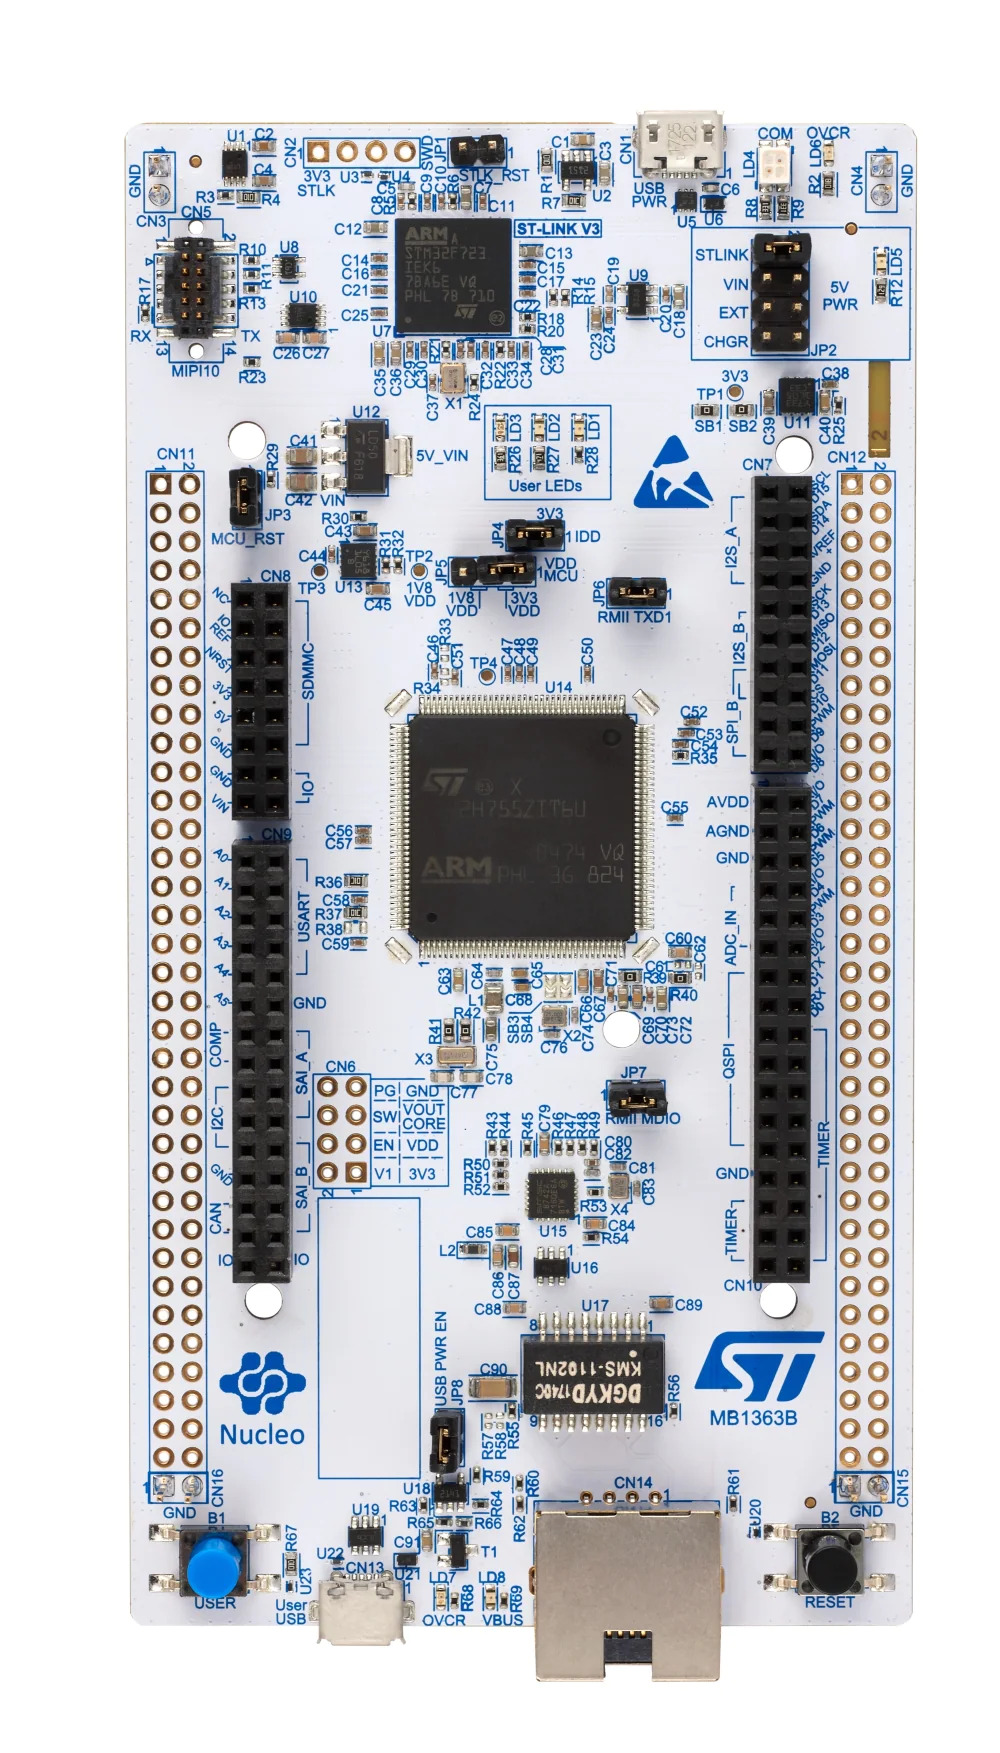
\includegraphics[height=150mm, keepaspectratio, angle=90]{figures/devboard.jpg}
    \caption{The STM32 Nucleo-H745 Development Board}
    \label{fig:Nucleo-H745}
\end{figure}

\section{Hardware Capabilities}

\subsection{Power}

Power can be provided to the MCU in a variety of ways and with different voltages ranging from 3.3 to 11 Volts. This makes it easy for developers to integrate this microcontroller into their designs. In this project, however, only the development board will be used. The easiest way to power the development board is through a micro USB port, which is also used for programming and debugging. As a connection to a PC is already needed in this early stage of development, the fact that power is also derived from this connection makes this setup comfortable to use or move.

\subsection{Clocks}

In the default setup, the MCU starts with an external clock signal that originates from the Board Management Controller. This controller is also responsible for programming and debugging. The microcontroller contains internal oscillators as well as PLLs. The usage of these can be configured in runtime during the setup phase of an application. Usually, in the first part of initializing the application the clock is set, in this case, a PLL will be used with the external clock signal from the Board Controller used as reference.

Several clock domains make it possible to fine-tune our application for low power consumption. Configuration code can be generated using official tools from the manufacturer using a GUI application. A maximum frequency of 480 MHz can be achieved for the M7 core and 240 MHz for the M4 core.

\subsection{Analog interfaces}

\subsubsection{Analog Digital Converter}

Almost all modern microcontrollers include some kind of analog-to-digital converter peripheral and the STM32H745 is not an exception \cite{ADCDescription}. It has three ADC-s where ADC1 and ADC2 are tightly coupled with ADC1 being the master while ADC3 is fully independent. Each ADC consists of a 16-bit successive approximation analog-to-digital converter and has up to 20 multiplexed channels. A/D conversion of the various channels can be performed in single, continuous, scan, or discontinuous mode. The result of the conversion is stored in a left-aligned or right-aligned 32-bit data register.

The ADC-s can use a lower resolution than 16-bit to decrease conversion time which is also independent of the AHB bus clock frequency. The ADCs are capable of self-calibration which reduces the complexity of their initialization. The start of a conversion can be initiated either by means of the software calling the applicable driver function, or hardware triggers, ie. interrupts of timer events. They are also capable of sending in interrupts themselves when a conversion is finished.

There are two main modes of using an ADC. The easiest method is using single conversion mode. With this mode, all the channel conversions are started and once these are finished, the results are stored in the appropriate registers and an end-of-conversion flag is checked. This way a blocking call to an ADC conversion can be easily implemented by waiting for the end of the conversion flag to be flipped. The second way is continuous conversion mode. Here, instead of stopping after the conversion is done and the result is placed in a register, the ADC will start this process again. When a conversion is finished it sends an interrupt that the data should be extracted from the register. Not handling this interrupt properly (ie. not saving the content of this register) will not stop the ADC from overwriting the content of the register.

The timing of a conversion can be useful information when designing an application. The elapsed time between the start of a conversion and the end of the conversion is the sum of the configured sampling time plus the successive approximation time depending on data resolution can be calculated according to the following formula.

\[T_{CONV} = T_{SMPL} + T_{SAR} = [1.5_{|min} + 7.5_{|14bit}] \times T_{adc\_ker\_ck}\]

\[ T_{CONV} = 62.5 ns_{|min} + 312.5 ns_{|14bit} = 375.0 ns\]

Where $T_{SMPL}$ is the sampling time which depends on the channel and $T_{SAR}$ depends on the resolution. In the formula above $T_{adc\_ker\_ck}$ equals 24 MHz, the resolution is 14-bit, and the lowest possible sampling time is substituted to demonstrate its usage.

\begin{figure}[H]
    \centering
    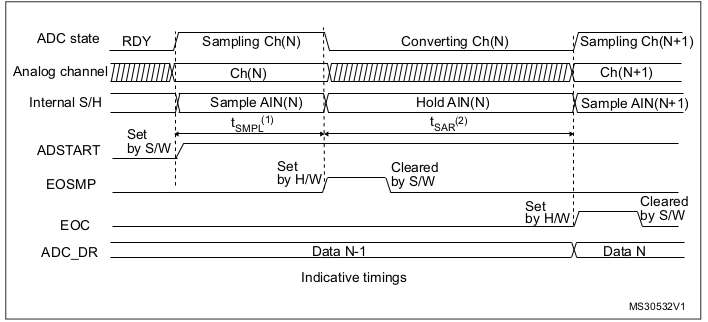
\includegraphics[width=150mm, keepaspectratio]{figures/adc-timing.png}
    \caption{Analog to Digital Conversion Timing\cite{ADConversionTime}}
    \label{fig:adc-timing}
\end{figure}

\subsubsection{Digital Analog Converter}

The DAC module is a voltage output digital-to-analog converter that can be configured in 8 or 12-bit mode. The DAC module has two output channels, and both of them have their converters. In dual DAC channel mode, conversions could be done independently or simultaneously when both channels are grouped for synchronous update operations \cite{DACDescription}.

There is one unified interface but two different DAC channels that can work in synchronized or independent modes. The DAC is able to generate noise-wave and triangular waves. They also have capabilities of using the DMA controller for their data buffers and using external triggers, ie. interrupts or timer events, for conversion is possible as well. The DAC can send interrupts to signal buffer underrun when using DMA mode but not in any other case.

When outputting a value, the DOR (Data Out Register) cannot be written directly, it should first be entered into the DHR (Data Hold Register). It is then automatically transferred to the DOR as soon as possible. This transfer is followed by a settling time which is dependent on the power supply voltage and the analog output load.

\begin{figure}[!ht]
    \centering
    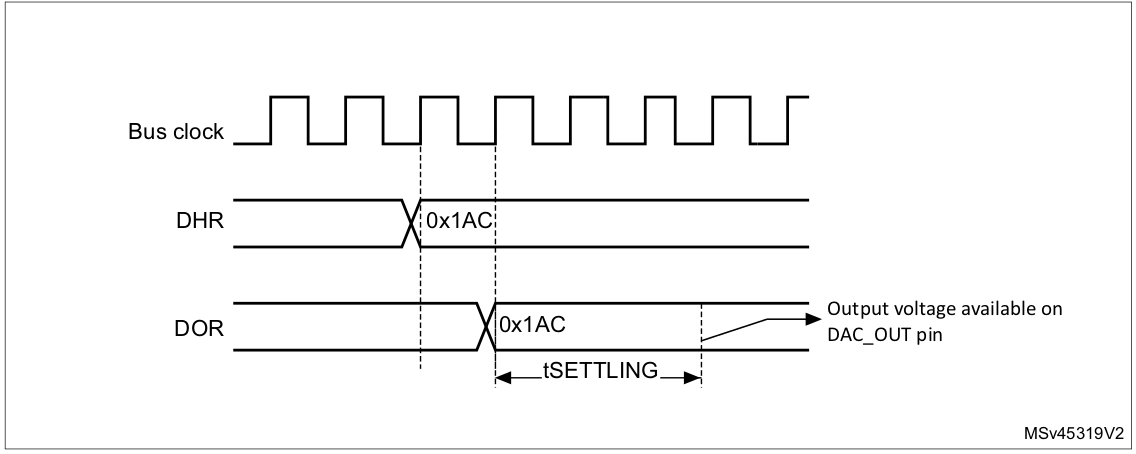
\includegraphics[width=150mm, keepaspectratio]{figures/dac-timing.png}
    \caption{Digital to Analog Conversion Timing\cite{DACTime}}
    \label{fig:dac-timing}
\end{figure}

In summary, the DAC has fewer features and fewer capabilities than the ADC on this microcontroller.

\subsection{Connectivity}

\subsubsection{Programming and debugging}

This development board is equipped with an on-board ST-LINK debugger and programmer. This module can handle the USB connection to a computer and also act as a virtual COM port or a debug port. There are multiple ways of programming the device using the ST-LINK connection, a programmer is available in the official STM IDE (Integrated Development Environment) but there are also standalone command line and GUI tools for programming. Any suitable debugger can connect to the debug port of the ST-LINK module, debugging will be described more in-depth in a further chapter.

\subsubsection{Ethernet}

Both cores of the microcontroller have pins that can be considered to use an ethernet interface. The development board has an ethernet connector that is compliant with the IEE-802.3-2002 standard. The ethernet connector is a really interesting feature for this project as in the second part when developing a more complex application. Such an application would be able to provide a minimal web GUI (Graphical User Interface) thanks to the ethernet connector.

\subsubsection{USB}

The development board has in total 2 USB Micro-AB connectors. One of them is connected to the previously mentioned ST-LINK connector so it cannot be configured freely. However, the other one is fully available for the programmer to use. Most likely this project will not utilize the USB port, but with similar complexity, and sometimes similar speeds, it could replace the ethernet port as another high-speed communication interface if needed.

\subsubsection{USART}

Multiple pins can be configured for USART peripherals, however the most important in this case is the one available through the \mycode{PD8} and \mycode{PD9} pins, which can be connected to the ST-LINK connector. By doing this we have a way of communicating with our program through a trivial communication protocol that requires minimal setup and driver support, and using the same USB port we used for powering and programming the board. Throughout development this port will be used for displaying debug traces.

\subsection{Other useful peripherals}

\subsubsection{GPIO-s}

As the pins of the STM32H745 MCU are very configurable and 144 pins are routed onto the development board, there is a considerable amount of GPIO-s that can be utilized if needed, though many of them are taken by other peripherals on the board. Three GPIO-s are each routed to a different colored user LED on the board, which is extremely useful in the early bring-up of a board as blinking an LED is often considered the "Hello World of hardware-related projects". Also present on the board are 2 buttons, one of which is a dedicated reset button while the other can be configured by the user.

\subsubsection{Hardware semaphores}

The hardware semaphore block on this system provides 32 32-bit register-based semaphores. The semaphores can be used to ensure synchronization between different processes running between different cores. They provide a non-blocking mechanism to lock semaphores in an atomic way even when multiple cores are trying to access them at the same time. There are two ways of locking one of these hardware semaphores. The first method is useful when not only the other core, but some other process from any core could try to access the semaphore. With this method, the \mycode{COREID} and \mycode{PROCID} are written to the semaphore, followed by a read check. A one-step lock is also available, where only the \mycode{COREID} is read from the semaphore.

The semaphores can generate an interrupt on any of the interrupt lines, this needs to be configured during the peripheral initialization phase. A semaphore is only cleared when \mycode{COREID} and \mycode{PROCID} match, except that a global clear is available per \mycode{COREID}. All 32 hardware semaphores have the following features: 8-bit PROCID, 4-bit COREID, 2 interrupt lines, and lock indication.

The semaphore is free when its LOCK bit is 0. In this case, the COREID and PROCID are also 0. When the LOCK bit is 1, the semaphore is locked and the COREID indicates which AHB bus master locked it. The PROCID indicates which process of that AHB (Advanced High-performance Bus) bus master locked the semaphore. When write-locking a semaphore, the COREID is taken from the master ID, and the PROCID is taken from the write data. When read locking the semaphore, the COREID is taken from the AHB bus master ID, and the PROCID is zero. There is no PROCID available with the 1-step (read) lock. The COREID is taken from the AHB bus master ID. The PROCID is written by the software of that AHB bus master. Each AHB bus master process must have a unique PROCID. PROCID is only available in the 2-step lock procedure.

\begin{figure}[!ht]
    \centering
    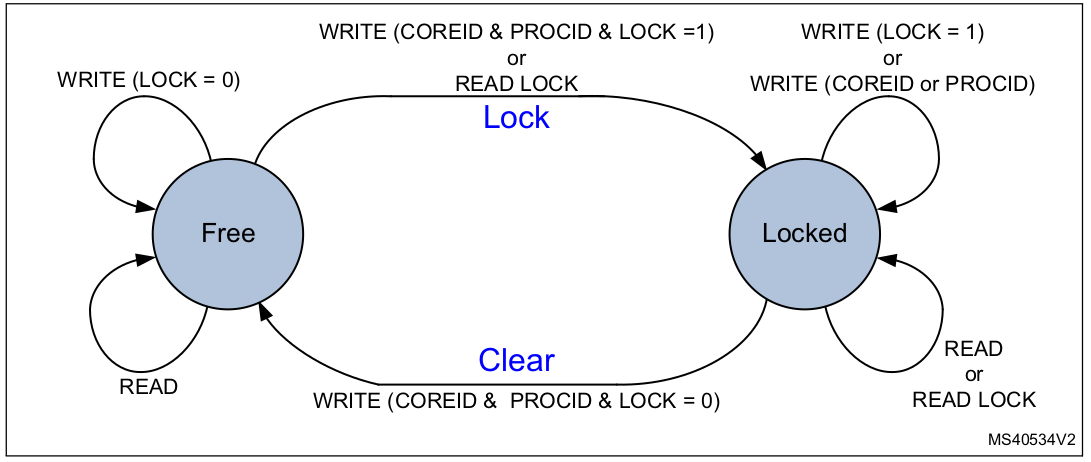
\includegraphics[width=150mm, keepaspectratio]{figures/hw-semaphore.png}
    \caption{Hardware semaphore state diagram \cite{HWSemaphore}}
    \label{fig:HWSemaphore}
\end{figure}

Clearing a semaphore is a protected process, to prevent accidental clearing by an AHB bus master or by a process that does not have the semaphore lock right. The semaphore clear procedure consists of writing to the semaphore with the corresponding COREID and PROCID and LOCK = 0. When cleared, the semaphore LOCK, the COREID, and the PROCID are all 0. When cleared, an interrupt may be generated to signal the event. To this end, the semaphore interrupt must be enabled.

%\include{content/latex-tools}
%\include{content/thesis-format}
%\include{content/template-usage}
%\include{content/task-interpretation}


% Acknowledgements
%~~~~~~~~~~~~~~~~~~~~~~~~~~~~~~~~~~~~~~~~~~~~~~~~~~~~~~~~~~~~~~~~~~~~~~~~~~~~~~~~~~~~~~
%%----------------------------------------------------------------------------
\chapter*{\koszonetnyilvanitas}\addcontentsline{toc}{chapter}{\koszonetnyilvanitas}
%----------------------------------------------------------------------------

I would like to express my deepest gratitude to my advisor, Dr. Tamás Kovácsházy, for his support and guidance during the time of this project and the my whole university journey. With his help on this project I was able to venture into a fascinating field of study that very much piqued my interest despite being relatively new.

I would also like to extend my heartfelt thanks to all my friends who supported me through ups and downs while enrolled in this master's degree program.

Finally, I extend my deepest gratitude to my mother, Zsuzsanna Katona, whose unwavering support and selfless encouragement have been a pillar of strength throughout my university journey.



% List of Figures, Tables
%~~~~~~~~~~~~~~~~~~~~~~~~~~~~~~~~~~~~~~~~~~~~~~~~~~~~~~~~~~~~~~~~~~~~~~~~~~~~~~~~~~~~~~
%\listoffigures\addcontentsline{toc}{chapter}{\listfigurename}
%\listoftables\addcontentsline{toc}{chapter}{\listtablename}


% Bibliography
%~~~~~~~~~~~~~~~~~~~~~~~~~~~~~~~~~~~~~~~~~~~~~~~~~~~~~~~~~~~~~~~~~~~~~~~~~~~~~~~~~~~~~~
\addcontentsline{toc}{chapter}{\bibname}
\bibliography{bib/mybib}


% Appendix
%~~~~~~~~~~~~~~~~~~~~~~~~~~~~~~~~~~~~~~~~~~~~~~~~~~~~~~~~~~~~~~~~~~~~~~~~~~~~~~~~~~~~~~
%----------------------------------------------------------------------------
\appendix
%----------------------------------------------------------------------------
\chapter*{\fuggelek}\addcontentsline{toc}{chapter}{\fuggelek}

The project is in a public repository available at: \newline\url{https://github.com/Goldan32/h745-start}

\setcounter{chapter}{\appendixnumber}
%\setcounter{equation}{0} % a fofejezet-szamlalo az angol ABC 6. betuje (F) lesz
\numberwithin{equation}{section}
\numberwithin{figure}{section}
\numberwithin{lstlisting}{section}
%\numberwithin{tabular}{section}


%\label{page:last}
\end{document}
